%----------------------------------------------------------------------------------------
%	SECTION 6
%----------------------------------------------------------------------------------------

\section{Additional General Skills (G)}


\subsection*{G1} \label{sec:G1}

% Please add the following required packages to your document preamble:
% \usepackage[table,xcdraw]{xcolor}
% If you use beamer only pass "xcolor=table" option, i.e. \documentclass[xcolor=table]{beamer}
\begin{wraptable}{r}{0.2\textwidth}
	\begin{tabular}{|c|}
		\hline
		\rowcolor[HTML]{F8A102}
		\textbf{G1} \master \\ \hline
		All courses and \\
		placements \\ \hline
	\end{tabular}
\end{wraptable}

I have had several opportunities to apply my skills in problem solving, communication, information retrieval, working with others and the effective use of general IT facilities.
I will demonstrate my application of these skills by providing examples from the work I produced for Sunamp and \textit{Climate Change, Sustainability and Adaptation} (\CCSA).
%A good example is when I applied these skills to produce the UniQ Overview Sheet, Product Selection Quiz and PISs for Sunamp (see \Cref{App:Overview,App:quiz,App:PISs}).
I applied my skills in:
\begin{itemize}
    \item Problem solving at Sunamp, as demonstrated in Section \ref{sec:quiz}, by solving the problem of guiding customers to their most suitable UniQ products through the creation of a quiz (see Appendix \ref{App:quiz}).
    %when I encountered inconsistencies or unclear information in the UniQ manuals.
    %For example, I was tasked with providing accurate and up-to-date dimensions of the UniQ batteries because the dimensions provided in the UniQ manuals were inconsistent.
    %Therefore, I asked a staff member what might be the cause for the discrepancy and they explained that the different dimensions might be referring to different UniQ prototypes.
    %They also suggested that I measure the batteries that were currently being mass-produced.
    %So I asked for a tape measure and used it to measure the dimensions of the most current UniQ batteries.
    %I also cross-checked my measurements with the staff member's until we settled on reasonable nominal dimensions.
    %As a result, I created a diagram with the nominal dimensions... 
    
    \item Communication during a recent D11CA assignment in which the aim was to write a POSTnote.
    POSTnotes are briefings on public policy issues that are based on academic and industrial research.
    They are written to inform the Parliamentary Office of Science and Technology (POST) so that appropriate policies can be developed.
	The crux of the assignment was to write technical information in layman's terms so that any politician could fully understand the issue at hand before entering a parliamentary debate or meeting.
	I wrote my POSTnote on adapting UK households to a 2050 climate and received a provisional mark of 67\%.
	My communication was successful, as my feedback reflects:
	``Overall, this is very clearly written and easy to understand."
    %as I produced the documents.
    %With the development of the quiz, I managed to come up with a way to efficiently direct customers to the most suitable UniQ product for them, which made the customers more informed and reduced the workload for the sales team.
    
    \item Information retrieval at Sunamp in order to produce accurate PISs (see Appendix \ref{App:PISs}).
    This was done by reading the UniQ manuals and other documents, doing online research and asking staff members for explanations to fill my gaps in understanding, and hands-on experience (e.g. measuring the dimensions of UniQ batteries).
    
    \item Working with others at Sunamp in order to produce the UniQ documents, which was a collaborative effort.
    (See Sections \ref{sec:quiz} and \ref{sec:piss} for references to collaborations and iterative feedback processes.)
    
    \item The effective use of general IT facilities at Sunamp throughout the production of the UniQ documents.
    For example, I would regularly print out my latest drafts for easy marking-up during meetings and back up my drafts online on Google Drive.
    I also applied this skill in D11CA by converting a Word document (docx) to a Portable Document Format (pdf) so that the POSTnote could be displayed consistently over different IT systems.
    %utilised media conversion techniques to ensure that the same message was displayed consistently over different IT systems
    % I created the Overview Sheet on Microsoft Publisher, the quiz on Microsoft PowerPoint, and the PISs on Microsoft Word. % MS applications are just software, not facilities.
\end{itemize}



\subsection*{G2}

\begin{wraptable}{r}{0.2\textwidth}
    \begin{tabular}{|ll|}
        \hline
		\rowcolor[HTML]{F8A102}
        \multicolumn{2}{|c|}{\textbf{G2} \nomaster} \\ \hline
        \ConTechTwo & \HYD \\
        \DPB & \CAS \\
        \DSA & \PC \\
        \EnBldgs & \TPS \\
        \DI & \PRJ \\
        \DST & \LAB \\
        \IP & \CCSA \\
        Arup & Hoare Lea \\
        Sunamp & Sweco \\
        \multicolumn{2}{|l|}{Hultin \& Lundquist} \\ \hline
    \end{tabular}
\end{wraptable}

\textit{N.B. For this LO, I have interpreted ``self-learning" as ``self-initiated learning", i.e. 
myself deciding and taking action to learn something that is not mandated by an external force,
%OR myself taking the initiative to learn something
whether I teach it to myself or somebody else teaches it to me.}

During my years at Heriot-Watt University, I have not initiated a personal project with the aim of learning something within a certain time frame.
Hence, I have not \emph{planned self-learning and improved performance} within a single project.
I would still consider myself to be a lifelong learner, though, as I have planned my self-learning and improved my performance on separate occasions.

%On the one hand, my personal programme of work that I used during my Dissertation (see Figure \ref{DST_schedule}) demonstrates my ability to plan self-learning.
%Moreover, my strategic approach to selecting optional courses and applying for placements demonstrates my ability to plan self-learning.
%in order to gain the most interesting and relevant knowledge to my course and gain exposure to different fields of work

On the one hand, my ability to \emph{plan self-learning} can be demonstrated by my personal programme of \DST \space work (see Figure \ref{DST_schedule}), as well as my strategic approach to selecting optional courses and applying for placements.
In Year 2, I selected \HYD \space and \DPB \space as I thought they would respectively deepen and develop my Architectural Engineering knowledge and design skills.
Since Year 2, also, I have tried to gain exposure to different fields of work through my summer placements.
Thus, I have so far experienced working in Mechanical Engineering, Architecture, Electrical Engineering, Environmental Building Certification, and Renewable Energy.

\begin{wrapfigure}{r}{0.4\textwidth}
	\centering
	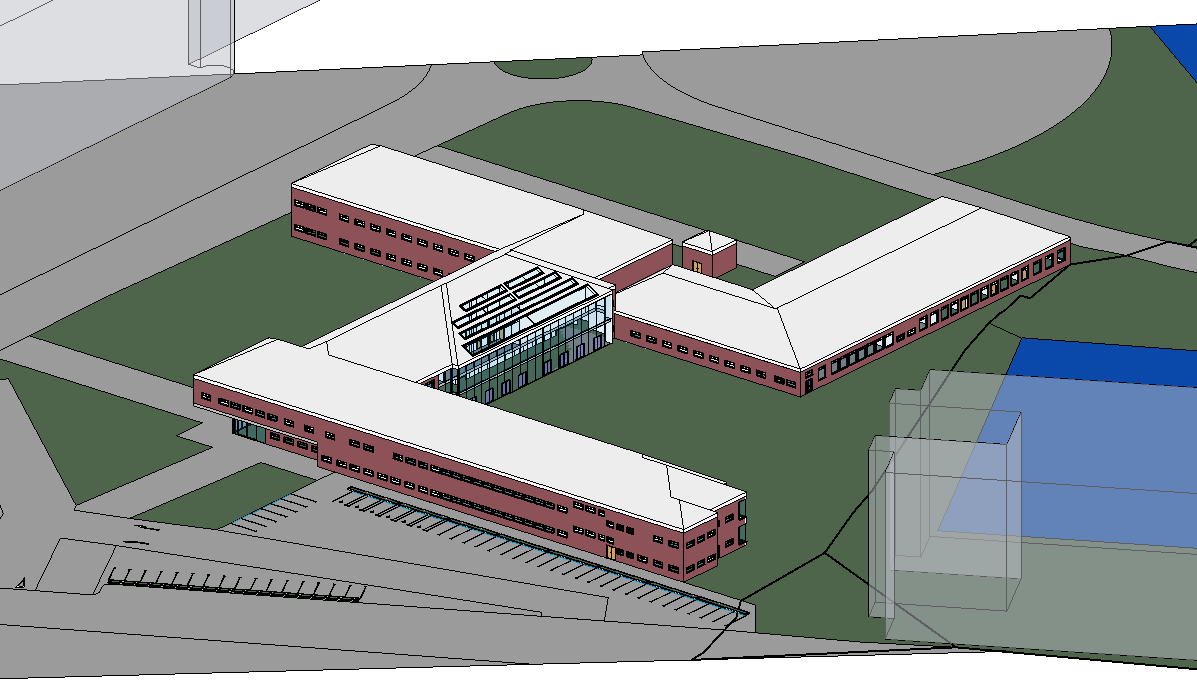
\includegraphics[width=0.4\textwidth]{figures/South.PNG}
	\rule{0.4\textwidth}{0.5pt} % use line???
	\caption{The building model I created in Revit for the \PRJTitle.}
	\label{fig:revit}
\end{wrapfigure}

On the other hand, I have self-learned to \emph{improve my performance} in certain IT skills, notably modelling in Revit and writing documents in LaTeX.
During the \PRJTitle, I attended Revit workshops that are provided on a weekly basis by the \deptname.
%(EGIS).
This learning experience improved my Revit modelling skills, enabling me to produce a building model for the \PRJTitle \space (see Figure \ref{fig:revit}).
As for LaTeX, since I was introduced to the document preparation system in Year 2, I have written most of my assignments in the system.
This has improved my ability to produce large professional-looking documents with reduced formatting-hassle (a problem I often experienced in Microsoft Word).
This report, for example, was written in LaTeX.




\subsection*{G3(i, b, m)}

\begin{wraptable}{r}{0.2\textwidth}
    \begin{tabular}{|ll|}
        \hline
        \rowcolor[HTML]{F8A102}
        \multicolumn{2}{|c|}{\textbf{G3(i, b, m)} \nomaster} \\ \hline
        \PRJ & \ISE \\
        \DST & \SIB \\
        \LAB & \ICP \\
        \multicolumn{2}{|c|}{Sunamp} \\ \hline
    \end{tabular}
\end{wraptable}

Throughout my years at Heriot-Watt University, I have increasingly planned and carried out a personal programme of work.
This culminated in Year 4, when we had the \textit{Design Project} and \textit{Dissertation} which were both long-term personal projects.
In the interim report that I wrote for my Dissertation, I included a personal programme of work (similar to a Gantt chart) that mapped out when and how I would work on the different sections of my dissertation for the rest of the academic year (see Figure \ref{DST_schedule01}).
I \emph{adjusted} the programme as I carried it out (see final programme in Figure \ref{DST_schedule02}) [\textbf{G3b}].
The major variations between the initial and final versions of the programme are:
\begin{itemize}
    \item No more work was done in Semester 1 and during the Christmas holidays. This was because I had decided that it was better for me to use that time to focus on my Design Project instead.
    \item The programme was more compressed, due to the above reasons.
    \item The blue block was segmented into two blocks. Blue represented my work on questionnaires and interviews. The gap was introduced to allow the respondents time to answer my survey before I interviewed them.
\end{itemize}

%\hl{Whereas I mostly assisted my supervisors with their projects at my other placements, the work I did at Sunamp was very much a personal project....}


\begin{figure}[htbp]
    \centering
        \begin{subfigure}{.45\textwidth}
          \centering
          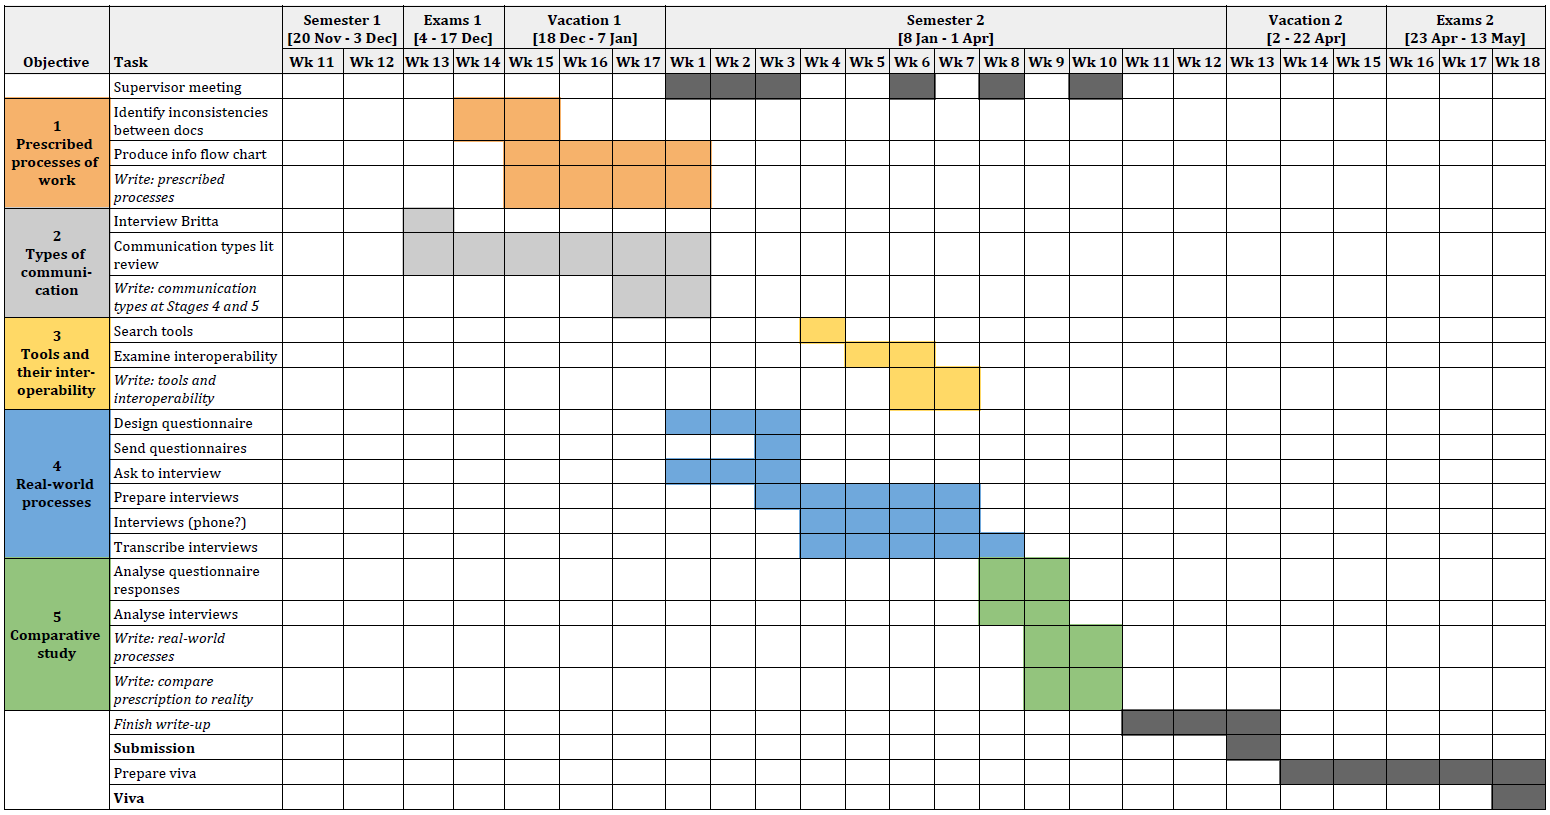
\includegraphics[width=\textwidth]{figures/DST-schedule-start.PNG}
%          \rule{\textwidth}{0.5pt} % use line???
          \caption{Initial programme}
          \label{DST_schedule01}
        \end{subfigure}
        \begin{subfigure}{.51\textwidth}
          \centering
          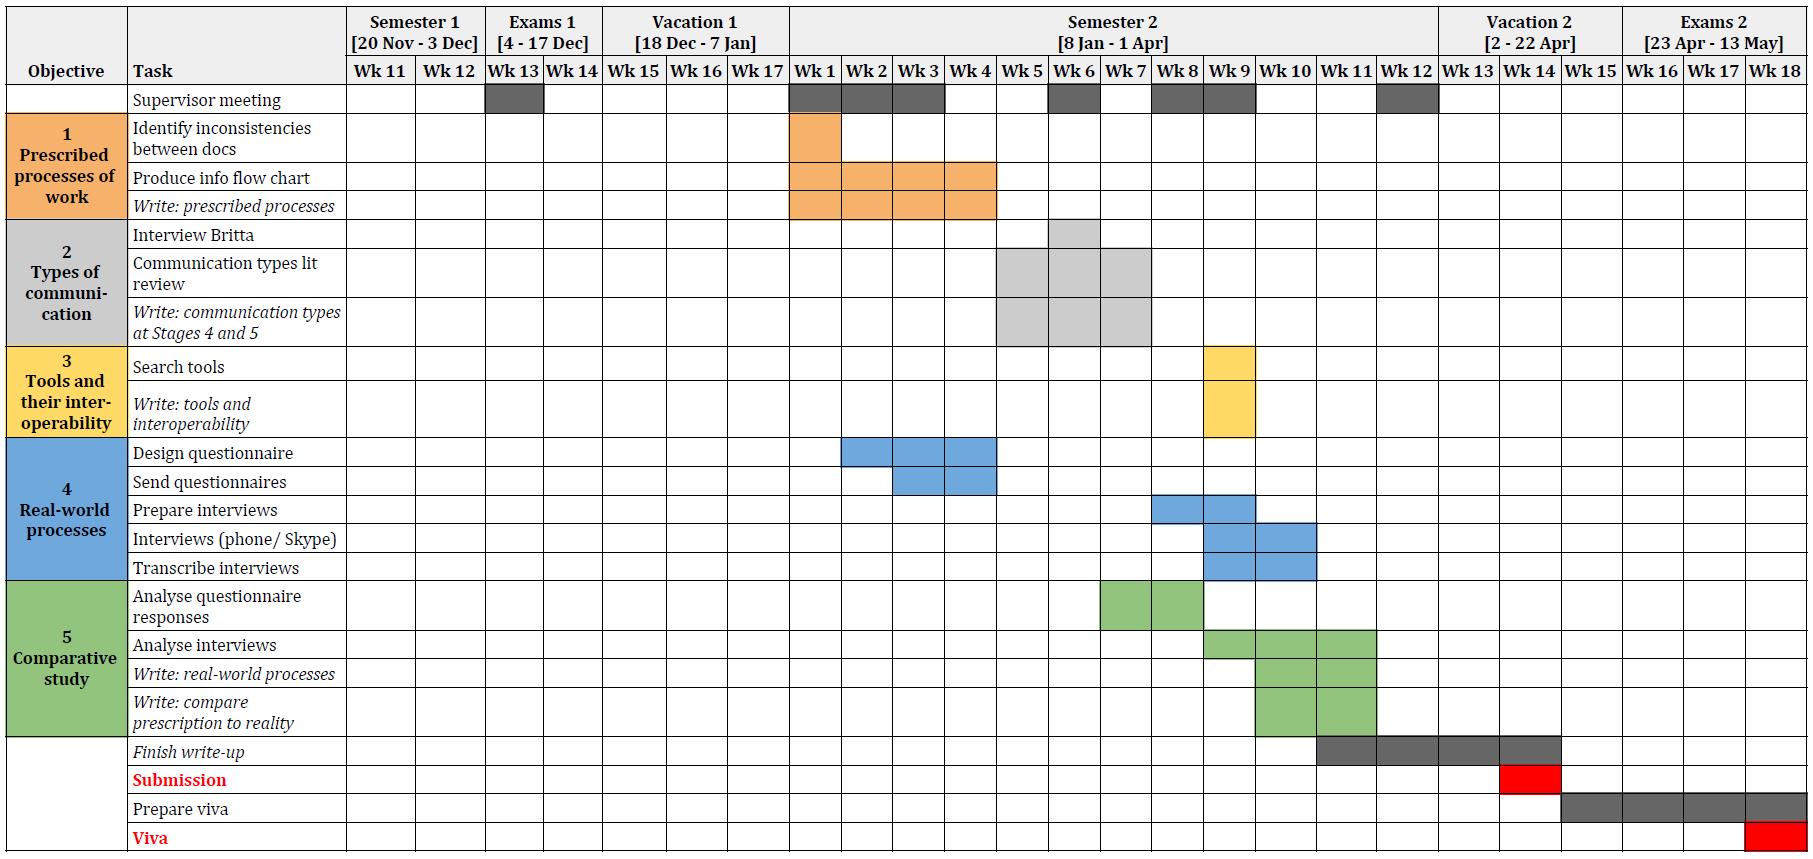
\includegraphics[width=\textwidth]{figures/DST-schedule-end-big.PNG}
%          \rule{\textwidth}{0.5pt} % use line???
          \caption{Final programme}
          \label{DST_schedule02}
        \end{subfigure}
    \rule{\textwidth}{0.5pt} % use line???
    \caption[My personal programme of work for my dissertation.]{My personal programme of work for my dissertation, from the end of Semester 1 to to the end of Semester 2 of Year 4.}
    \label{DST_schedule}
\end{figure}


\begin{wrapfigure}{r}{0.5\textwidth}
	\centering
	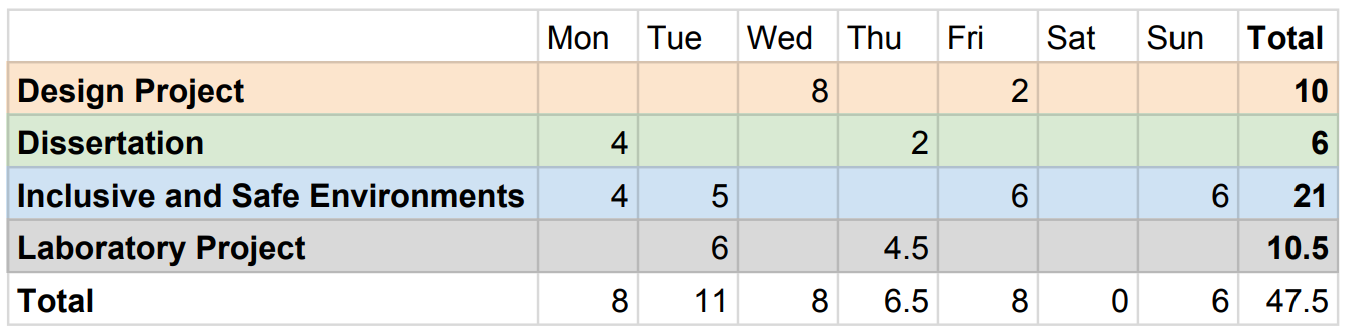
\includegraphics[width=0.5\textwidth]{figures/y4s1w6hours.PNG}
	\rule{0.5\textwidth}{0.5pt} % use line???
	\caption{Time log from Week 6 of Semester 1, Year 4.}
	\label{fig_timelog}
\end{wrapfigure}

In Year 4, I also started to \emph{monitor} the hours I worked in order to \emph{adjust} and improve my personal programme \emph{on an on-going basis} [\textbf{G3m}].
Figure \ref{fig_timelog} provides an example of my weekly time log from Year 4.
By monitoring the hours I worked, I noticed a trend: I typically worked fewer hours on Thursdays than any other day.
I proceeded to identify the reason for this, which is that I tended to feel tired or burnt out by that day of the week.
After this discovery, I allocated myself less hours to work and focused on less demanding tasks (if possible) on Thursdays.
The hours that I lost on Thursday I would then try to compensate for throughout the rest of the week.




\subsection*{G4(i, -)}

\begin{wraptable}{r}{0.2\textwidth}
    \begin{tabular}{|ll|}
        \hline
        \rowcolor[HTML]{F8A102}
        \multicolumn{2}{|c|}{\textbf{G4(i, -)} \master} \\ \hline
        \ID & \IE \\
        \EnvBeh & \CAS \\
        \EnBldgs & \TPS \\
        \DI & \FMP \\
        \PRJ & \LAB \\
        \ISE & \CCSA \\
        Arup & Hoare Lea \\
        Sunamp & Sweco \\
        \multicolumn{2}{|l|}{Hultin \& Lundquist} \\ \hline
    \end{tabular}
\end{wraptable}

My degree programme and my work placements have provided me with multiple opportunities to work as part of a team.
In all of the projects, I have exercised personal responsibility, and sometimes also initiative, as a team member.
For example, the work I produced for Sunamp, including the quiz I came up with (see Section \ref{sec:sunamp_work}), is a display of me exercising initiative and my personal responsibility to the company.

In most academic projects, however, I have exercised personal responsibility, and sometimes initiative, as a team leader.
% Sometimes this has involved me exercising initiative also.
A recent example of this is a group project of creating and presenting a poster for \textit{Climate Change, Sustainability and Adaptation}.
I assumed a leading role in this group mainly by coordinating the group activity (e.g. arranging and leading meetings, setting up weekly agendas).
For this project, I sketched the drawing in Figure \ref{fig:Sketch01} and suggested the use of such an image to graphically show the importance of our topic.
After the group agreed on its usefulness to the poster, I went ahead and developed a final version (see Figure \ref{fig:Sketch02}).
This was an act of initiative because the use of a representative image had previously not been discussed within the group.


\begin{figure}[htbp]
    \centering
        \begin{subfigure}{.49\textwidth}
          \centering
          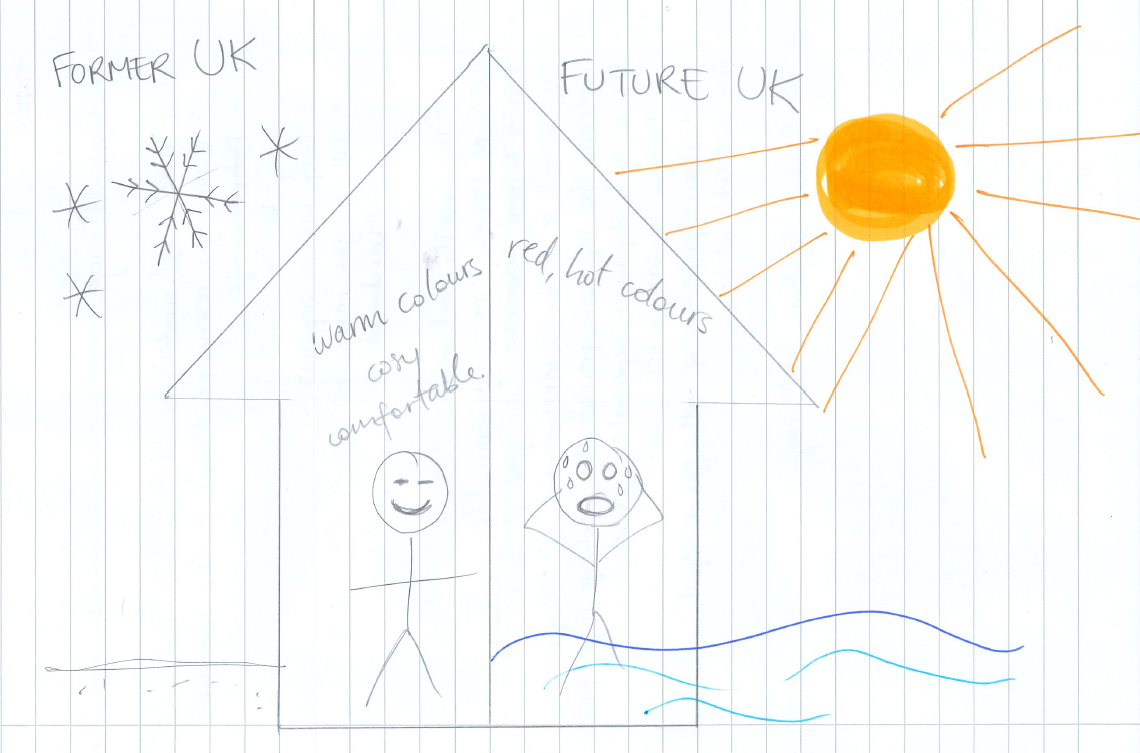
\includegraphics[width=\textwidth]{figures/sketch.PNG}
%          \rule{\textwidth}{0.5pt} % use line???
          \caption{Initial sketch}
          \label{fig:Sketch01}
        \end{subfigure}
        \begin{subfigure}{.47\textwidth}
          \centering
          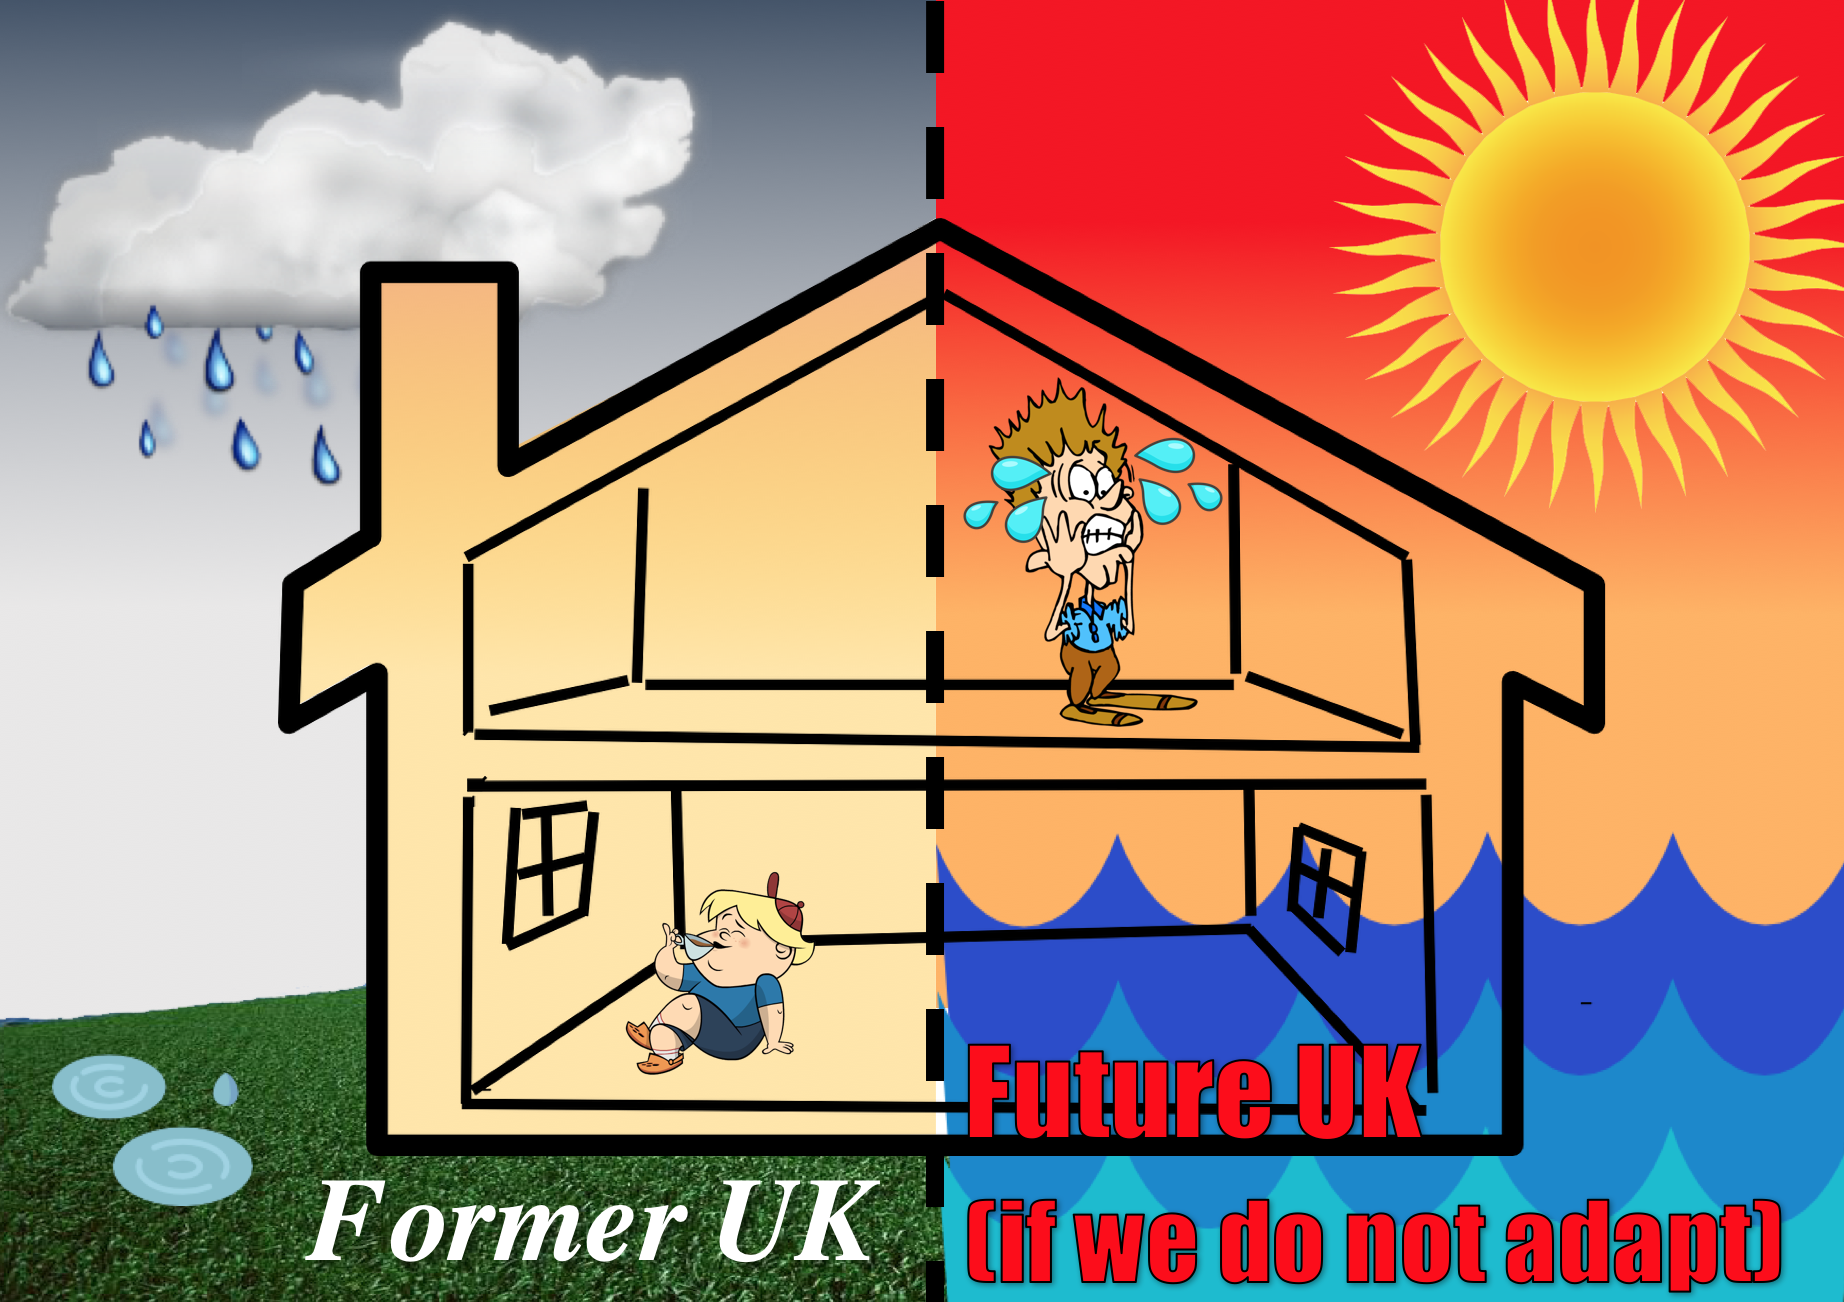
\includegraphics[width=\textwidth]{figures/eposter_sketch_2.png}
%          \rule{\textwidth}{0.5pt} % use line???
          \caption{Final image}
          \label{fig:Sketch02}
        \end{subfigure}
    \rule{\textwidth}{0.5pt} % use line???
    \caption[\CCSA poster image.]{The image I suggested and developed to use on a group poster to show the importance of adapting UK houses to future climate impacts.}
    \label{fig:Sketch}
\end{figure}